\chapter{Reliability in SCDTs}
\label{reliability}

\section{Cached Nack Reliability}
Just like in traditional Internet services, IoT applications have a variety of
reliability constraints.  We propose that in a SCDT, the reliability should be
constructed using negative acknowledgments (``nacks") from children.  Previous
research has already shown the negative acknowledgment scheme to be superior to
regular acknowledgments in traditional network-level multicast trees
\cite{SRM, RFC3208}; we argue that this principle extends to SCDTs.
Unlike these previous schemes, SCDTs utilize caching at intermediate nodes.  We
argue that drafting intermediate routers as caches will improve scalability (by
reducing the amount of traffic that must flow to the root) and improve partition
tolerance (since retransmission could still occur even if the path to the root
is lost).  We call this scheme Cached Nack Reliability (CNR).

The SCDT forwards data unreliably to improve latency, but caches the data it
forwards at each intermediate node.  A traditional simple nacking scheme could use a similar method to that employed in TCP \cite{RFC0793}: by examining an incrementally increasing sequence number associated with the SCDT included with every packet.  Gaps observed in the sequence numbers of received packets indicate what data to nack.  Periodic heartbeats sent by child nodes and acknowledged by parents keep sequence numbers updated even when data isn't frequently published.  However, we argue for a more complex method: including a byte offset and packet length in the header of each packet.  This method supports refragmentation of packets at intermediate points in the network.

Leaves can determine their reliability constraints for themselves, and send a
nack for the missing data to their parent.  If there is a cache hit, the data is
retransmitted; if there is a miss, the nack is forwarded to the leaf's
grandparent and so on, ultimately creating a hierarchy of caches.  A slightly
more sophisticated scheme could use timers with exponential backoff to reduce
unnecessary and redundant nacking \cite{SRM, RFC3208}.  Since we are
arguing for a reliable system and the scheme presented so far relies on caches,
there must ultimately be one or more places in the network where data is durably
stored when caches all miss; 
see~\autoref{durability-replication} for more
details.

Such a scheme provides a best of both worlds solution, minimizing latency while
supporting packet retransmission.  It breaks the
traditional reliable vs unreliable (generally TCP vs UDP) trade off developers
must choose between.  By putting the impetus to nack packets on the leaf, rather
than being completely reliable or unreliable, a leaf node could set a level of
unreliability.  For instance, a leaf node could choose to nack just enough
packets to maintain a particular record reception rate.


\section{Evaluation}
\label{cnr-eval}
We utilize a naive multicast tree building protocol to build the underlying multicast tree for our CNR tests. This allows us to evaluate CNR independently of SCDTs. In summary, the algorithm works as follows:

\begin{enumerate}  
	\item A joining node contacts the root and requests to join the tree. 
	\item The root pings the joining node to determine its round trip latency. 
	\item If the latency is substantially shorter than its existing children (or if the root has fewer children than \texttt{MAX\_FANOUT}), the root adds the joining node as a direct child. If not, the root sends back a list of its children.
	\item The joining node pings all of the children to determine which has the lowest latency.
	\item The joining node repeats the process with the closest (determined by round trip time) child. The process is repeated until the joining node finds a parent that will accept it.
\end{enumerate}

We evaluate CNR in comparison to another baseline algorithm. Our naive reliability algorithm simply uses TCP links between every parent and child, essentially creating a series of point-to-point TCP links. Our results are predicated on comparing this naive baseline to CNR. 

Using point-to-point TCP presents a number of issues in actual deployments. One is the risk of bottlenecking the entire tree due to one bad link, where a router's buffer becomes full and must drop incoming packets because it cannot push out data to one of its children fast enough. Another issue is the high computational cost of setting up TCP links, which is non-ideal if the tree is continuously shifting and re-optimizing. While we don't advocate using point-to-point TCP in multicast trees, it is a useful contrast point because it represent a fairly direct comparison to reliability in the unicast space.

Preliminary simulation results for CNR are generated on a star topology with the root in the center, using the naive trees (not SCDTs). Because of the limited fanout  of our trees, we nonetheless still build meaningful multicast trees on this topology.  See~\autoref{simulations} for more information about our simulation environment.  Link speeds are randomized to between 1 and 100 Mbps, and delays are randomized to between 1 and 100 ms.

\begin{figure}[h]
	\begin{center}
		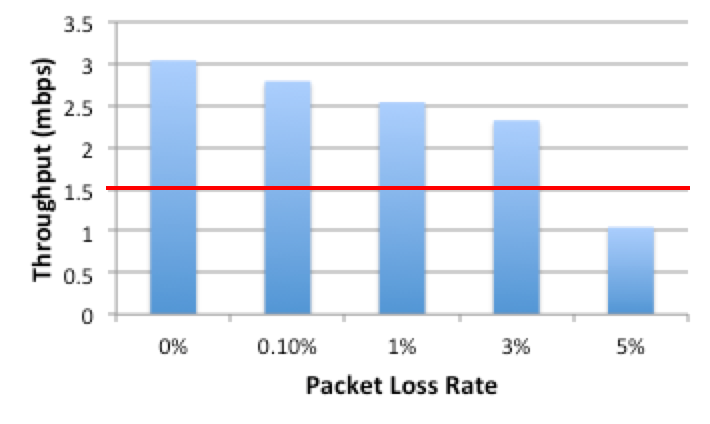
\includegraphics[scale=0.6]{cnr_bar.png}
		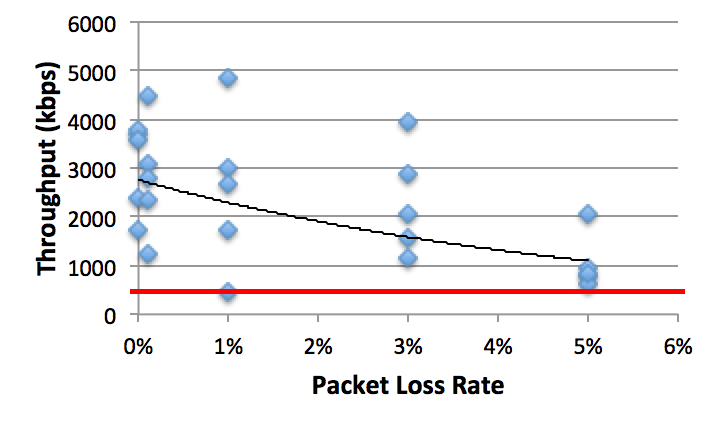
\includegraphics[scale=0.6]{cnr_scat.png}
	\end{center}
	\vspace{-1.3em}
	\caption{\small \itshape Impact on throughput of packet loss rate using CNR. Sampled by sending 100KB to a tree containing 50 subscribers and a \texttt{MAX\_FANOUT} of 4. The red line represents the average throughput of TCP over several runs with no packet loss.  Left: The average throughput of CNR over multiple runs. Right: The average throughput of CNR plotting individual runs and an exponential trend line.}
	\vspace{-1em}
	\label{fig:cnr_through}
\end{figure}

Our results are summarized in~\autoref{fig:cnr_through}. We sent 100KB of data to all the subscribing nodes in our multicast tree, and measured the throughput. We then introduced packet drops into the network, and measured the throughput of CNR when packets were randomly dropped 0.1\%, 1\%, 3\%, and 5\% of the time. The data suggests that CNR performs well in the face of fairly substantial packet loss, with fairly minor performance degradation until packet losses grow above 3\%, after which performance reductions become more substantial. 

What is particularly interesting, however, is how much better CNR performed compared to hop-to-hop TCP links, even with no packet loss. Our data shows CNR generating substantially greater throughput than hop-to-hop TCP even when CNR is experiencing 3\% packet loss and TCP is experiencing none; the breakeven point is somewhere between 3\% and 5\% packet loss. While this is admittedly hardly the use case TCP was designed for, we believe this demonstrates the superiority of our approach and of nacking in multicast applications in general. We attribute the poor performance of hop-to-hop TCP to the overhead imposed by the TCP protocol and the loss of end-to-end efficiency \cite{end-to-end-args} TCP generally relies on. As discussed in~\autoref{architecture}, however, using many end-to-end TCP connections simply does not scale with the number of subscribers we are considering.

We believe this result will only improve with increased scale. Our test described  in~\autoref{fig:cnr_through} considers only 50 nodes and a \texttt{MAX\_FANOUT} of 4, meaning that a packet would traverse at most 3 overlay hops to reach its destination. In a larger network (or, in some cases, in an SCDT), the number of hops would be greatly increased. In a system without caching, this would impose substantially greater round trip times. However, we did not test the effect of varying cache sizes and the impact of cache misses on CNR performance.
